\section{Semi-Analytical Primal Solver}
\label{sec:sap_solver}

Our Semi-Analytical Primal Solver, or SAP for short, essentially is a Newton
iteration used to find the minimum of the unconstrained formulation stated in
Eq. (\ref{eq:primal_unconstrained}), where constraints have been eliminated
using our analytical inverse dynamics, and thus the name of the solver.

Though this new problem is strictly convex and can be solved using Newton's method
we make the following observations
\begin{enumerate}
	\item Since projections $P_\mathcal{F}$ are continuous, we will see when
	computing gradients, that not only the cost $\ell_p(\mf{v})$ is continuous,
	but also its gradient.
	\item The Hessian $\mf{H}=\nabla^2\ell_p$ is piecewise continuous, with
	large variations of \textit{curvature}. While this is not a problem for
	Newton's method given its \textit{affine invariance} property in theory, in
	practice we will use an analytically computed Hessian to avoid numerical
	round-off errors.
	\item\label{item:line_sarch} Since the problem is strictly convex, line
	search combined with Newton's method leads to guaranteed convergence.
	However, given the large variations in curvature, in practice we find that a
	specially designed exact line search performs best.
\end{enumerate}

Item \ref{item:line_sarch} is of utmost important in practice. We'll show a
strategy that allows to perform line search with machine precision. A
careful pre-computation of commonly occurring terms enable us to perform this
step for a small fraction of the total cost. While machine precision is
not required in practice, we show that the cost to achieve this level of
convergence is negligible and it is well worth it for a robust implementation
that can handle very stiff systems (with small regularization).

In the next subsections we describe each component of the solver in detail.

\subsection{Gradients}
\label{sec:gradients}

We summarize the main results required for implementation. Detailed derivations
are provided in the Appendix \ref{app:gradients_derivation}. We will see that in
order to compute both the gradient and Hessian of the cost we only need
analytical expressions of the projection $P_\mathcal{F}$ and its gradient.

The gradient of the primal cost $\ell_p$ is
\begin{equation}
	\nabla_\mf{v}\ell_p(\mf{v}) = \mf{A}(\mf{v}-\mf{v}^*) + \nabla_\mf{v}\ell_R
\end{equation}

Computing this gradient might seem a daunting enterprise, but after substitution
of $\nabla_\mf{v}P_\mathcal{F}$ the result is beautifully simple
\begin{equation}
	\nabla_\mf{v}\ell_p(\mf{v}) = \mf{A}(\mf{v}-\mf{v}^*) - \mf{J}^T\bgamma(\mf{v})
	\label{eq:primal_gradient}
\end{equation}
with $\bgamma(\mf{v})$ from the analytical inverse dynamics. This recovers the
original momentum balance in Eq. (\ref{eq:momentum_linearized}) since Newton's
method solves for $\nabla_\mf{v}\ell_p=\mf{0}$.

Notice tha the gradient in Eq. (\ref{eq:primal_gradient}) is continuous since
the projection in the analytical inverse dynamics in Eq.
(\ref{eq:analytical_y_projection}) is continuous.

We obtain the Hessian $\mf{H}=\nabla_\mf{v}^2\ell_R$ by taking the gradient of
Eq. (\ref{eq:primal_gradient}). The result is
\begin{eqnarray}
	\nabla_\mf{v}^2\ell_R(\mf{v}) &=&
	\mf{J}^T\mf{G}\,\mf{J}\nonumber\\
	\mf{G} &=& \nabla_{\mf{v}_c}\bgamma = -\nabla_\mf{y}\bgamma \mf{R}^{-1}
	\label{eq:ellR_hessian}
\end{eqnarray}
where $\nabla_{\mf{v}_c}\!\bgamma$ is a block diagonal matrix where each
diagonal elements is the $3\times 3$ matrix
$\nabla_{\mf{v}_{c,k}}\!\bgamma_k$ for the $k\text{-th}$ contact. As shown in
Appendix \ref{app:gradients_derivation}, $\nabla_{\mf{v}_c}\bgamma\succeq 0$ and
thus $\nabla_\mf{v}^2\ell_R(\mf{v})\succeq 0$.

Finally, the Hessian needed in Newtons's method is
\begin{equation}
	\mf{H}= \mf{A} + \mf{J}^T\mf{G}\,\mf{J}
	\label{eq:ell_hessian}
\end{equation}
which, since $\mf{A}\succ 0$, is strictly positive definite. We note however that
showing $\mf{H}\succ 0$ is not enough for $\ell_p$ to be
strictly convex. Since $\nabla_\mf{v}\ell_p$ is a piecewise function, we must
additionally require that the directional derivative across the boundary
$\partial\mathcal{F}$, of $\mathcal{F}$ increases. Formally, if $\mf{\nu}$ is
the normal to $\partial\mathcal{F}$, then we require
\begin{equation}
	\frac{\partial \ell_p^-}{\partial \nu} \le \frac{\partial \ell_p^+}{\partial \nu}
\end{equation}
we show this to be the case in Appendix \ref{app:gradients_derivation} which
then leads to the confirmation that $\mf{H}\succ 0$.

\RedHighlight{Question to Frank: what's the easiest way to show that
$\ell_p(\mf{v})$ is convex? vs. my approach of showing that the Hessian is
piecewise convex.}

\subsection{Newton iteration}
\label{sec:solver_details}

With the analytical expressions for both the gradient and Hessian of
$\ell_p(\mf{v})$, we use Newton's method to find the unique minimum of Eq.
(\ref{eq:primal_unconstrained}). At each $k\text{-th}$ iteration we
compute a search direction according to
\begin{equation}
	\Delta\mf{v}^{k+1} = -\mf{H}^{-1}(\mf{v}^k)\nabla_\mf{v}\ell_p(\mf{v}^k)
	\label{eq:Newton_iteration}
\end{equation}

Since the problem is convex, we can perform a line search along this direction
to find the global minimum. At each Newton iteration, the line search solves the
one-dimensional minimization problem
\begin{eqnarray}
	\alpha = \argmin_{t\in\mathbb{R}^{++}} \ell_p(\mf{v}^k + t \Delta\mf{v}^{k+1})
	\label{eq:line_search_optimization}
\end{eqnarray}
and the iteration is updated as $\mf{v}^{k+1}=\mf{v}^{k} + \alpha
\Delta\mf{v}^{k+1}$.

Specifics of the line search algorithm are critical to the success of the SAP
solver given that the Hessian can undergo large changes as $\mf{v}^k$ explores
states corresponding to different contact modes. We tried two line search
strategies that we describe next.

\subsection{Inexact Line Search}
Most if not all mature solver implementations that use Newton's method solve Eq.
(\ref{eq:line_search_optimization}) only approximately.

Our implementation explores values in a geometric sequence $\alpha_{m} = \rho^m$
with $\rho \in (0, 1)$ until Armijo's criteria is satisfied, i.e.
$\ell_p(\alpha_m) < \ell_p(\alpha^k) + c\,\alpha_m d\ell_p/d\alpha(\alpha^k)$.
We typically use $\rho=0.8$ and $c=10^{-4}$. We refer to this procedure as the
\textit{inexact} method to differentiate it from our exact (modulo round-off
errors) line search described next. Armijo's rule allows to prove convergence of
Newton's method, see \RedHighlight{Cite here, possibly best book by Michel
Bierlaire}.

\subsection{Exact Line Search}
Given that $\ell_p$ might exhibit steep gradients, we found out that the
accuracy of the inexact line search can lead to a large number of Newton
iterations.
Therefore we propose an exact method that uses a fast computation of the
first and second derivatives of $\ell_p$ to drive a local one-dimensional Newton
method. We make the following additional observations
\begin{enumerate}
	\item $\ell_p(\alpha)$ is strictly convex, i.e. there is a unique minimum.
	\item Since $\ell_p(\alpha)$ is strictly convex, a Newton step is guaranteed
	to be well formed given that $d^2\ell_p/d\alpha^2>0$.
	\item $\ell_p(\alpha)$ is a piecewise $C^1$ function. In other words,
	$d\ell_p/d\alpha$ is continuous but $d^2\ell_p/d\alpha^2$ might not be.	
	\item Given the regularization used to model friction and stiff compliance,
	gradients of $\ell_p(\alpha)$ can undergo large changes, even within a
	region where $\ell_p(\alpha)$ is continuous.
\end{enumerate}

This led us to choose a one-dimensional strategy that is robust under these
conditions. We found the method \verb;rtsafe; in \cite[\S
9.4]{bib:numerical_recipes} to work the best. \verb;rtsafe; is one-dimensional
root finder that uses the Newton-Raphson method and switches to bisection
whenever Newton's method leads to an iterate outside a search bracket or
whenever its convergence is slow. Using analytical first and second derivatives,
our line search simply reduces to finding the unique root of $d\ell/d\alpha$
using the \verb;rtsafe; algorithm. We found this method to perform so well, that
we iterate $\alpha$ to a machine precision at a negligible impact on the
computational cost. This allow us to use very tight regularization parameters
without having to tune tolerances in the line search.

\subsection{Efficient Analytical Derivatives For Line Search}

\verb;rtsafe; requires the first and second derivatives of
$\ell_p$, while the inexact method only requires the first derivative to verify
Armijo's stopping criteria. We show how to compute these gradients efficiently
in $\mathcal{O}(n)$ operations.

Defining $\ell(\alpha) = \ell_p(\mf{v}+\alpha\Delta\mf{v})$ we can
compute first and second derivatives with respect to $\alpha$ using the gradient
and Hessian
\begin{eqnarray}
	\frac{d\ell}{d\alpha}&=&\Delta\mf{v}^T\nabla_\mf{v}\ell(\alpha)\nonumber\\
	\frac{d^2\ell}{d\alpha^2}&=&\Delta\mf{v}^T\nabla_\mf{v}^2\ell(\alpha)\Delta\mf{v}\nonumber
\end{eqnarray}

These are expensive to compute derivatives for general non-linear functions and
most line search variations in practice are approximations that avoid their
computation altogether. We show that first and second derivatives can be
computed efficiently given the structure of the problem.

Using the gradients from Section \ref{sec:gradients} we can write
\begin{eqnarray}
	\frac{d\ell_M}{d\alpha}(\alpha)&=&\Delta\mf{v}^T\mf{A}(\mf{v}(\alpha)-\mf{v}^*)\\
	\frac{d\ell_R}{d\alpha}(\alpha)&=&-\Delta\mf{v}^T\mf{J}^T\bgamma
\end{eqnarray}
and defining the change of constraint velocity
$\Delta\mf{v}_c=\mf{J}\Delta\mf{v}$ and change of momentum $\Delta\mf{p} =
\mf{A}\Delta\mf{v}$ we obtain the much simpler and faster to compute versions
\begin{eqnarray}
	\frac{d\ell_M}{d\alpha}(\alpha)&=&\Delta\mf{p}^T(\mf{v}(\alpha)-\mf{v}^*)\\
	\frac{d\ell_R}{d\alpha}(\alpha)&=&-\Delta\mf{v}_c^T\bgamma(\alpha)
\end{eqnarray}
which only require dot products that can be computed in $\mathcal{O}(n_v)$ and
$\mathcal{O}(n_c)$ respectively.

Using the same definitions we can write simple expressions for the second
derivatives as well
\begin{eqnarray}
	\frac{d^2\ell_M}{d\alpha^2}(\alpha)&=&\Delta\mf{v}^T\mf{A}\Delta\mf{v}=\Delta\mf{v}^T\Delta\mf{p}\\
	\frac{d^2\ell_R}{d\alpha^2}(\alpha)&=&-\Delta\mf{v}_c^T
	\nabla_{\mf{v}_c}\bgamma\Delta\mf{v}_c
\end{eqnarray}
where notice that $\frac{d^2\ell_M}{d\alpha^2}$ is independent of $\alpha$ and
can be precomputed before proceeding into the line search and
$\frac{d^2\ell_R}{d\alpha^2}$ only involves $\mathcal{O}(n_c)$ operations given
the structure of $\nabla_{\mf{v}_c}\bgamma$, a block diagonal matrix.

\subsection{Problem Sparsity}

The sparsity patterns of the Hessian matrix in Eq. (\ref{eq:ell_hessian}) will
be described through an example. We will describe in general the sparsity of a
multibody system as a collection of \text{tree structures}, or a
\textit{forest}. Consider the system in Fig. (\ref{fig:sparsity_example}).
\begin{figure}[!h]
	\centering
	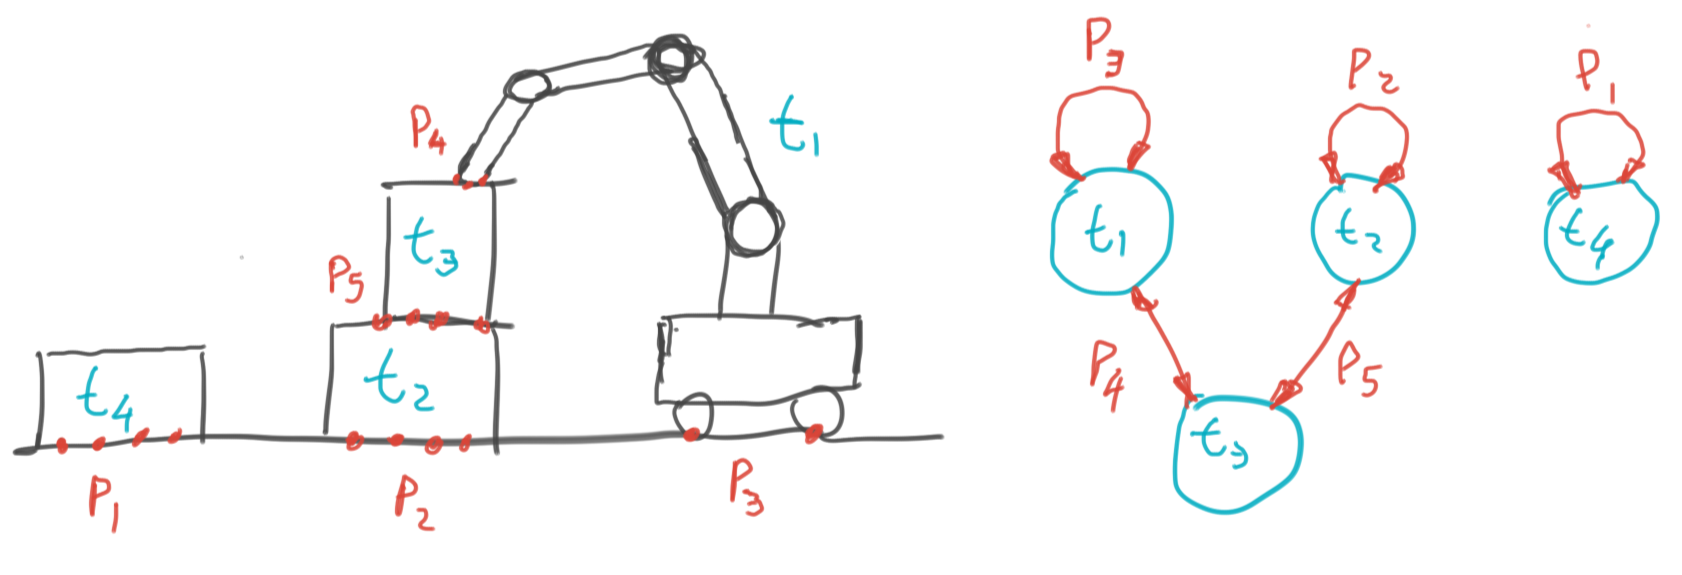
\includegraphics[width=0.7\columnwidth]{figures/sparsity_example.png}
	\caption{\label{fig:sparsity_example} 
	Example used to describe sparsity patterns commonly encountered in the
	simulation of robotic mechanical systems. The graph on the right puts
	\textit{trees} as nodes and contact \textit{patches} as edges. Notice how
	this graph exactly describes the sparsity pattern of the matrix
	$\mf{J}^T\mf{G}\mf{J}$ in Eq. (\ref{eq:JTGJ_sparsity}).}
\end{figure}
In this example a robot arm mounted on a mobile base constitutes its own tree,
here labeled $t_1$. The number of degrees of freedom of the $t\text{-th}$ tree
will be denoted with $n_t$. A free body is a special case of a tree where
$n_t=6$, this is a very common case. In general the mass matrix will have a
block diagonal structure where the $t\text{-th}$ diagonal block corresponds to
the mass matrix of the $t\text{-th}$ tree. For the example in Fig.
(\ref{fig:sparsity_example}) the mass matrix will look like\\\\
\begin{equation}
	\mf{M}=\quad
	\begin{bmatrix}
		\tikzmark{M_topleft}
		\diagentry{\mf{M}_{\cc{11}}}&&&\tikzmark{M_topright}\\
		&\diagentry{\mf{M}_{\cc{22}}}\\
		&&\diagentry{\mf{M}_{\cc{33}}}\\		
		\tikzmark{M_bottomleft}&&&\diagentry{\mf{M}_{\cc{44}}}
	\end{bmatrix}
% Draw lil arrows on top and to the left.
\tikz[overlay,remember picture] {
	\draw[->,thick,color=cyan]
  ([yshift=3ex]M_topleft) -- ([yshift=3ex]M_topright) node[midway,above]
  {\scriptsize $t$}; 
  \draw[->,thick,color=cyan]
  ([yshift=1.5ex,xshift=-2ex]M_topleft) -- ([xshift=-4ex]M_bottomleft)
  node[near end,left] {\scriptsize $t$};}	
\end{equation}

In general, we define as \textit{patches} as a collection of contact pairs
between the same two trees. We label in red all contact patches in Fig.
(\ref{fig:sparsity_example}). Each pair will correspond to a single cone
$k\text{-th}$ constraint in our contact formulation. The set of constraint
indexes $k$ that belong to patch $p$ is denoted with $\mathcal{I}_p$ of size
(cardinality) $|\mathcal{I}_p| = r_p$.

Notice that our definition of \textit{patches} as used here to describe sparsity
has nothing to do with the actual geometrical topology of the contact surface
between two trees. That is, the \textit{patches} as defined here, could in
general correspond to a simple connected surface or even a complex contact area
formed by a set of disconnected surfaces. Figure (\ref{fig:sparsity_example})
labels trees and patches and shows the corresponding graph where the nodes are
the trees and the edges are the contact patches.

Recall from Eq. (\ref{eq:ellR_hessian}) that $\mf{G} = \nabla_{\mf{v}_c}\bgamma$
is a block diagonal matrix, with $\mf{G}_k = \nabla_{\mf{v}_{c,k}}\bgamma_k \in
\mathbb{R}^{3\times 3}$ at the $k\text{-th}$ diagonal block. We can write this
also as $\mf{G} = \text{diag}(\mf{G}_p)$ if we group contact pairs by patches to
define $\mf{G}_p=\text{diag}(\mf{G}_k), \,\forall k\in\mathcal{I}_p$.

The contact Jacobian will in general be a sparse since the relative velocity at
a contact pair $k$ will only involve the generalized velocities of the trees in
contact. For the case in Fig. (\ref{fig:sparsity_example}) the Jacobian will
look like\\\\
\begin{equation}
	\mf{J}=\quad
	\begin{bmatrix}
		\tikzmark{J_topleft}\mf{0} & 
		\mf{0} & \mf{0} & \mf{J}_{\rr{1}\cc{4}}\tikzmark{J_topright}\\		
		\mf{0} & \mf{J}_{\rr{2}\cc{2}} & \mf{0} & \mf{0}\\
		\mf{J}_{\rr{3}\cc{1}} & \mf{0} & \mf{0} & \mf{0}\\
		\mf{J}_{\rr{4}\cc{1}} & \mf{0} & \mf{J}_{\rr{4}\cc{3}} & \mf{0}\\
		\tikzmark{J_bottomleft}
		\mf{0} & \mf{J}_{\rr{5}\cc{2}} & \mf{J}_{\rr{5}\cc{3}} & \mf{0}		
	\end{bmatrix}
% Draw lil arrows on top and to the left.
\tikz[overlay,remember picture] {
	\draw[->,thick,color=cyan]
  ([yshift=3ex]J_topleft) -- ([yshift=3ex]J_topright) node[midway,above]
  {\scriptsize $t$}; 
  \draw[->,thick,color=red]
  ([yshift=1.5ex,xshift=-3ex]J_topleft) -- ([xshift=-3ex]J_bottomleft)
  node[near end,left] {\scriptsize $p$};}	
\end{equation}
where each non-zero block is the Jacobian $\mf{J}_{\rr{p}\cc{t}}$ of size
$3r_p\times n_t$.

We have now the elements to describe the sparsity of the product
$\mf{J}^T\mf{G}\mf{J}$ in Eq. (\ref{eq:ell_hessian}). For the example in Fig.
(\ref{fig:sparsity_example}) this is
\begin{equation}
	\mf{J}^T\mf{G}\mf{J}=\quad
	\begin{bmatrix}
		\tikzmark{JTGJ_topleft}
		\JTGJ{3}{1}{1} + \JTGJ{4}{1}{1} & \mf{0} & \JTGJ{4}{1}{3} & \mf{0}
		\tikzmark{JTGJ_topright}\\		
		\mf{0} & \JTGJ{2}{2}{2} + \JTGJ{5}{2}{2} & \JTGJ{5}{2}{3} & \mf{0}\\
		\JTGJ{4}{3}{1} & \JTGJ{5}{3}{2} & \JTGJ{4}{3}{3} + \JTGJ{5}{3}{3} & \mf{0}\\
		\tikzmark{JTGJ_bottomleft}
		\mf{0} & \mf{0} & \mf{0} & \JTGJ{1}{4}{4}\\
	\end{bmatrix}
	\label{eq:JTGJ_sparsity}
% Draw lil arrows on top and to the left.
\tikz[overlay,remember picture] {
	\draw[->,thick,color=cyan]
  ([yshift=3ex]JTGJ_topleft) -- ([yshift=3ex]JTGJ_topright) node[midway,above]
  {\scriptsize $t$}; 
  \draw[->,thick,color=cyan]
  ([yshift=1.5ex,xshift=-2.5ex]JTGJ_topleft) -- ([xshift=-13ex]JTGJ_bottomleft)
  node[near end,left] {\scriptsize $t$};}	
\end{equation}

Notice how the sparsity pattern of $\mf{J}^T\mf{G}\mf{J}$ exactly matches the
graph from Fig. (\ref{fig:sparsity_example}). Moreover, given blocks $\mf{G}_p$
are symmetric, so is the product $\mf{J}^T\mf{G}\mf{J}$.

Finally the Hessian will have the sparsity structure of $\mf{A} +
\mf{J}^T\mf{G}\mf{J}$. \RedHighlight{Frank: for now, for rigid body dynamics, we
can assume $\mf{A}=\mf{M}$, the mass matrix. I'll see how to update the text to
reflect that. At least I believe this is ok as a good start for us to talk about
this.}


\subsection{Termination Conditions}
\RedHighlight{Write this section}